\documentclass[../../main.tex]{subfiles}

\begin{document}

fcaR\cite{doc4}  Es un paquete de R que permite aplicar Análisis de Conceptos Formales Difuso desde R, este paquete permite trabajar con contextos formales, extraer su retículo de conceptos y generar implicaciones a partir de ella.

Si abrimos el entorno de desarrollo RStudio y introducimos la siguiente matriz 

\begin{lstlisting}
x <- matrix(c(0, 1, 1, 0, 1,
              1, 0, 1, 1, 0,
              1, 1, 1, 1, 0,
              1, 0, 0, 1, 0,
              1, 1, 1, 1, 0,
              1, 0, 1, 1, 0), 
            nrow = 6, 
            ncol = 5, 
            dimnames = list(c("o1","o2","o3","o4","o5","o6"), c("a1","a2","a3","a4","a5")))
\end{lstlisting}

\vskip 0.2in

Podemos generar un contexto formal de dicha matriz con los siguientes comandos:
\begin{lstlisting}[mathescape]
fc <- FormalContext$\mbox{\textdollar}$new(x)
fc$\mbox{\textdollar}$find_concepts()
fc$\mbox{\textdollar}$concepts$\mbox{\textdollar}$plot()
\end{lstlisting}

\vskip 0.2in

\newpage

Al ejecutar el último comando se puede apreciar que se obtiene el mismo resultado que la figura anterior:
\begin{figure}[h]
\centering
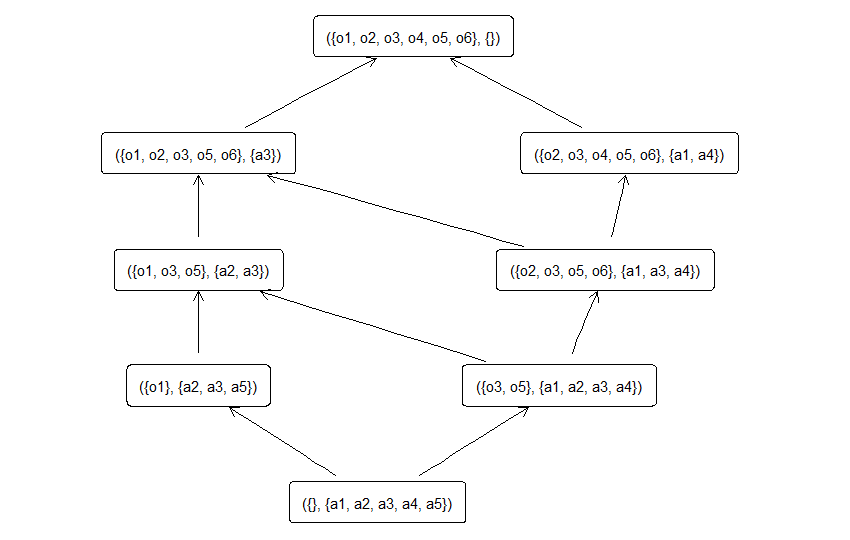
\includegraphics[width=1\textwidth]{images/3_fca/reticulo2.png}
\caption{Retículo de conceptos generado por fcaR del Ejemplo 1}
\end{figure}

\vskip 0.2in

Una vez generado el contexto formal con sus correspondientes conceptos es posible generar implicaciones del retículo de conceptos, es decir, al generar las implicaciones podemos encontrar relaciones entre los datos, si se ejecuta los siguientes comandos bajo el contexto formal generado anteriormente:

\vskip 0.2in

\begin{lstlisting}[mathescape]
fc$\mbox{\textdollar}$find_implications()
fc$\mbox{\textdollar}$implications$\mbox{\textdollar}$print()
\end{lstlisting}

\vskip 0.2in
\newpage
Se obtienen 4 implicaciones

\begin{lstlisting}
Implication set with 4 implications.
Rule 1: {a5} -> {a2, a3}
Rule 2: {a4} -> {a1}
Rule 3: {a2} -> {a3}
Rule 4: {a1} -> {a4}
\end{lstlisting}

\vskip 0.2in

dónde nos indica que:

\begin{itemize}
    \item El atributo $a5$ esta relacionado con los atributos $\{ a2,a3 \}$.
    \item El atributo $a4$ esta relacionado con los atributos $\{ a1 \}$.
    \item El atributo $a2$ esta relacionado con los atributos $\{ a3 \}$.
    \item El atributo $a1$ esta relacionado con los atributos $\{ a4 \}$.
\end{itemize}

\end{document}